The user should expect to input desired commands, controls, and specific
settings such as temperature and length of time by a easily through web interface. 
The user can expect that whichever temperature they set for their desired
application, that the temperature will remain constant.

\subsection{Programmable HLT Heating Element Temperature Management}
\subsubsection{Description}

The heating element on the HLT will need to maintain the temperature that is set
by the user via the web interface. The reason for customizable temperature is due to the varying
temperature requirements set by the recipe chosen by the user. This temperature control will be
managed by an ESP32 microcontroller. The temperature of the vessel will be
monitor by a DS18B20 digital thermometer. The microcontroller will take
continuous readings from the thermometer. When it begins dropping below the
desire temperature, the microcontroller will send a signal to a MOSFET relays. When the
relay receives that signal, it switch states and allow for power to be delivered
to the heating element. Once the desired temperature is reached, the
microcontroller will send another signal to the MOSFET relays. The relay will then
turn off, and this would turn off the power to the heating element.

\begin{figure}[H]
	\centering
	\graphicspath{.\images}
	\fbox{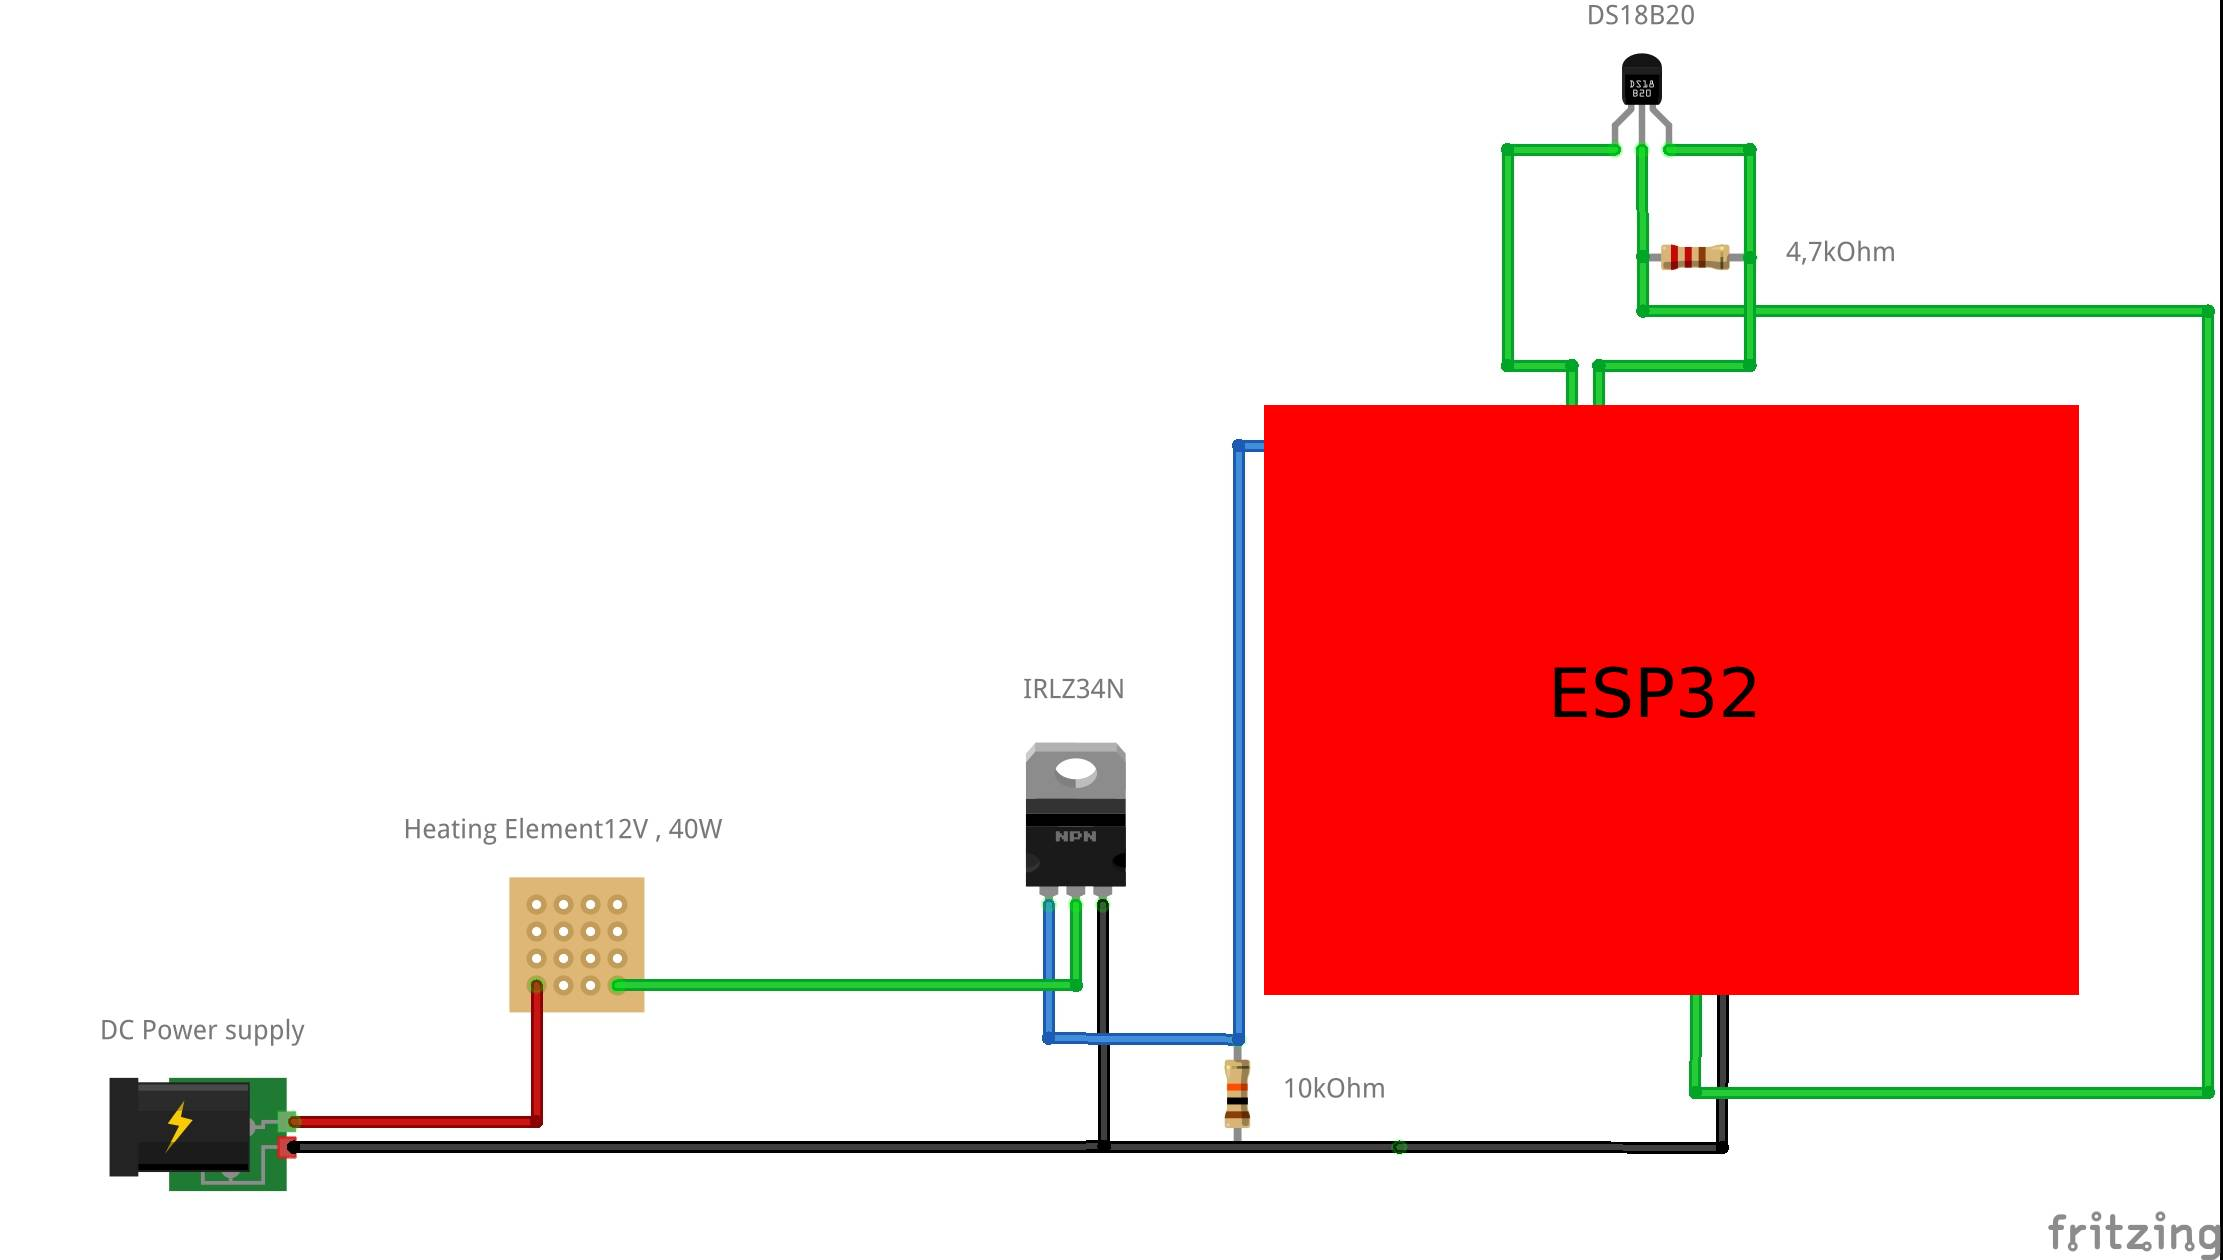
\includegraphics[scale=0.5]{images/temperature_control_diagram.jpg}}
	\caption{HLT Temperature Controller Diagram}
\end{figure}

\subsubsection{Source}
This requirement came from Dr. Chris Conly. He requested that our team enable
the user to be able to set a specific temperature via the web interface. The water is to stay at a constant boiling temperature to maximize
effectiveness of the mashing process.  
\subsubsection{Standards}
\begin{itemize}
\item IEC 60730
\item IEC 60335
\item EN ISO 13849
\end{itemize}
\subsubsection{Priority}
This feature is of \textbf{Critical} priority. Without this feature, we would be unable to
accomplish an effective mashing process. 

\subsection{Boiling Kettle Heating Element Temperature Management}
\subsubsection{Description}
The heating element on the boil vessel will need to maintain a water temperature of
212 degrees fahrenheit for optimal extraction. This temperature control will
managed by an ESP32 microcontroller. The temperature of the vessel will be
monitor by a DS18B20 digital thermometer. The microcontroller will take
continuous readings from the thermometer. When it begins dropping below the
desire temperature, the microcontroller will send a signal to a MOSFET relays. When the
relay receives that signal, it switch states and allow for power to be delivered
to the heating element. Once the desired temperature is reached, the
microcontroller will send another signal to the MOSFET relays. The relay will then
turn off, and this would turn off the power to the heating element.

\begin{figure}[H]
	\centering
	\graphicspath{.\images}
	\fbox{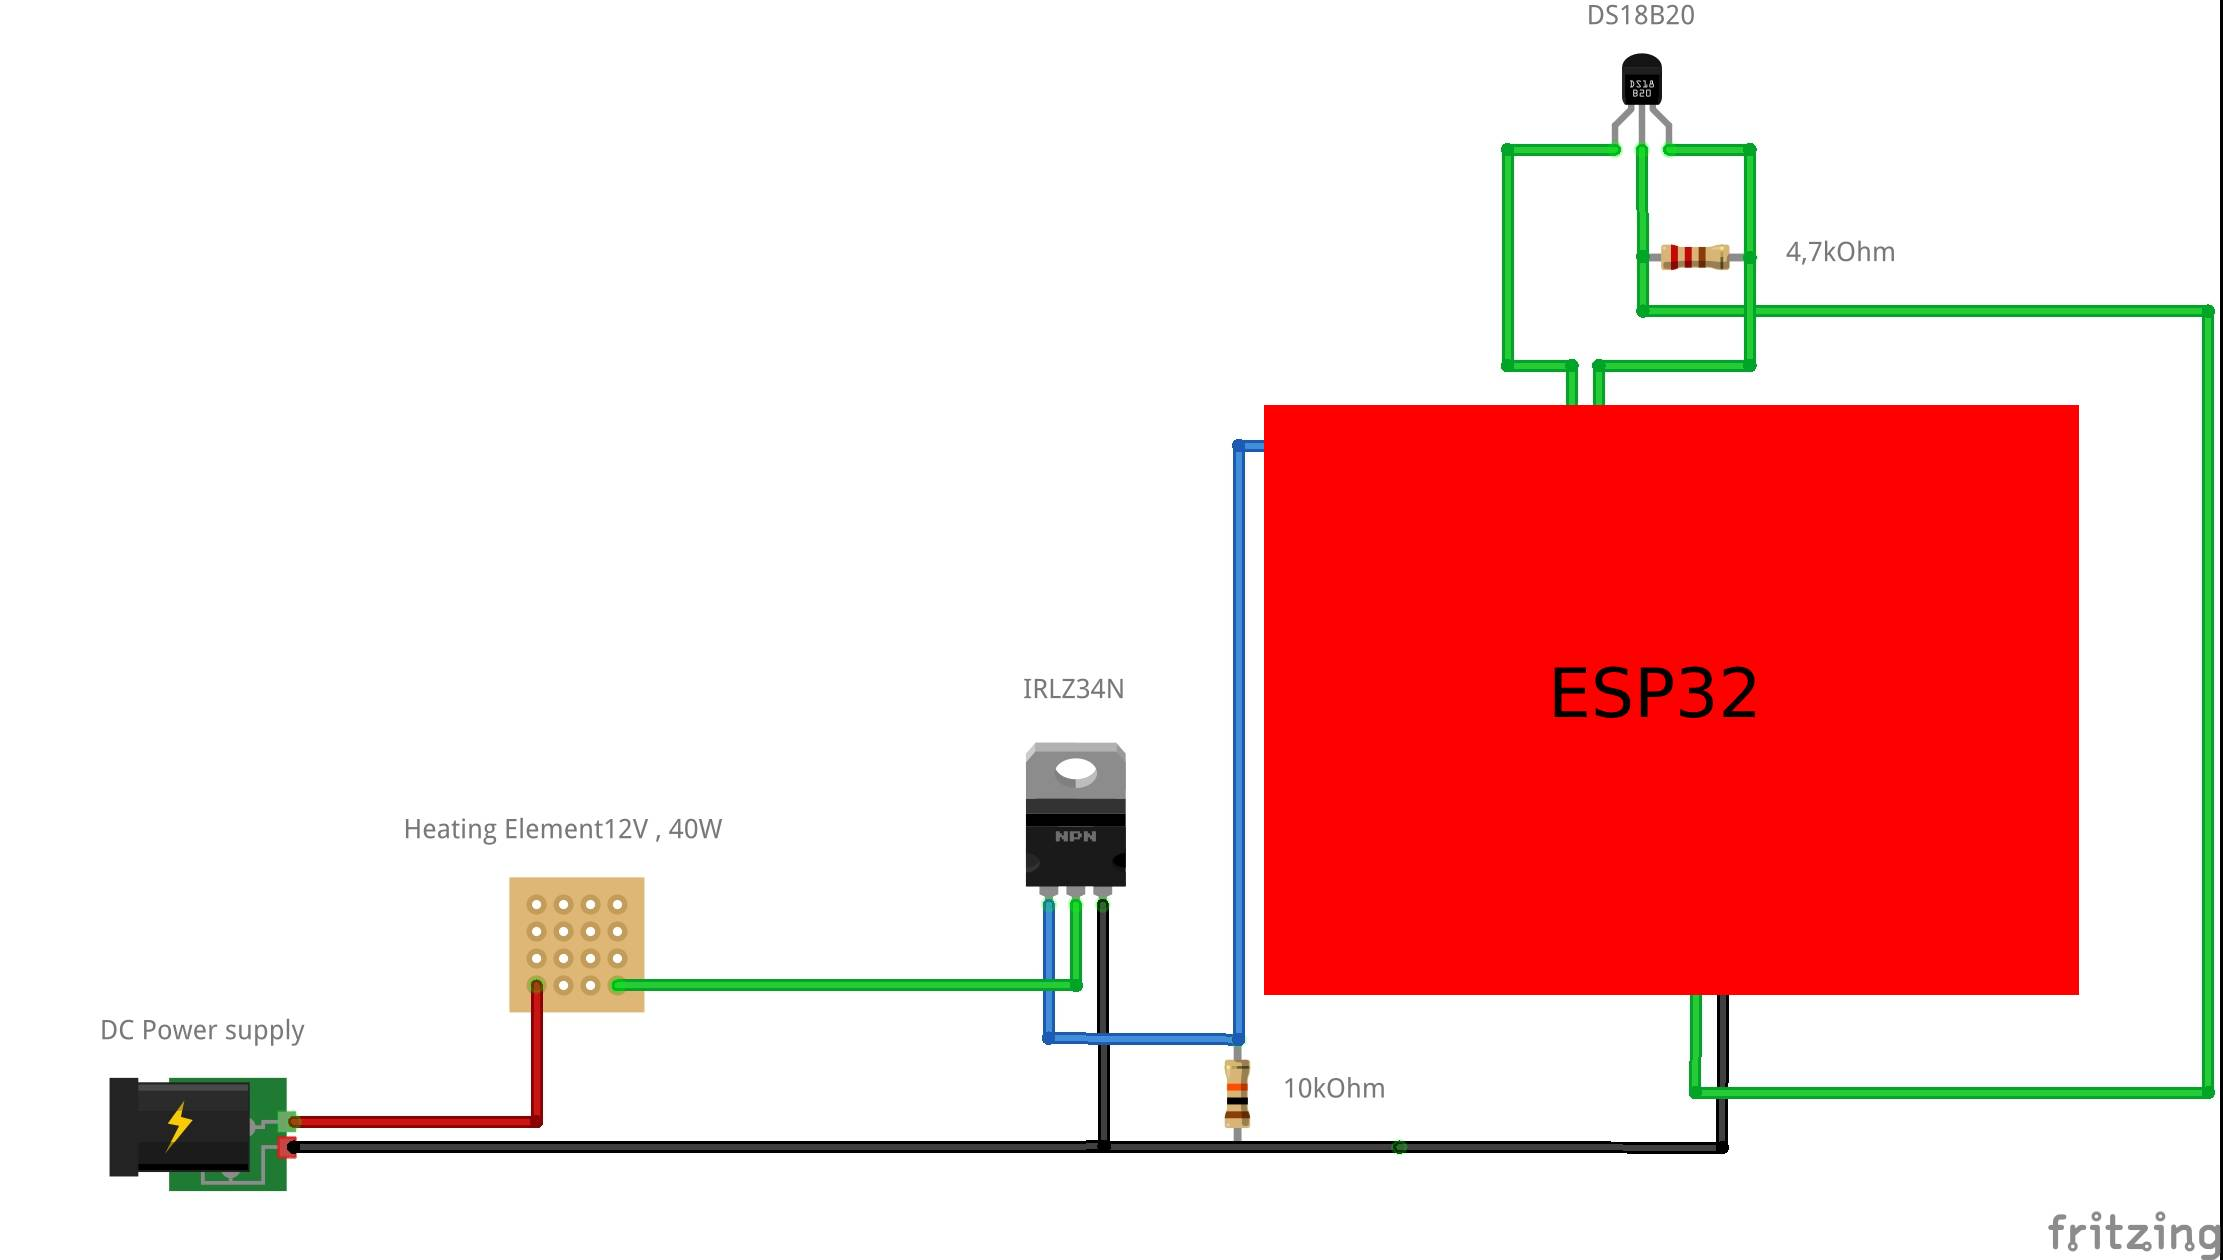
\includegraphics[scale=0.5]{images/temperature_control_diagram.jpg}}
	\caption{Boiling Kettle Temperature Controller Diagram}
\end{figure}

\subsubsection{Source}
This requirement came from Dr. Chris Conly. He requested that our team ensure
that the water stay a constant boiling temperature to maximize extraction.  
\subsubsection{Constraints}
Detailed description of applicable constraints...
\subsubsection{Standards}
\begin{itemize}
\item IEC 60730
\item IEC 60335
\item EN ISO 13849
\end{itemize}
\subsubsection{Priority}
This feature is of \textbf{Critical} priority. Without this feature we would be unable to
accomplish any sort of extraction. 
